\begin{figure}[htb]
\centering
\subfloat[The chair.]{\label{fig:chair}
{\parbox{2.5cm}{
\begin{tikzpicture}[scale = 10]
\tikzstyle{VertexStyle}=[shape = circle,	
								 minimum size = 1pt,
								 inner sep = 1.2pt,
                         draw]
\Vertex[x = 0.236114323139191, y = 0.890571415424347, L = \tiny {$y_1$}]{v0}
\Vertex[x = 0.238114297389984, y = 0.800571441650391, L = \tiny {$y_2$}]{v1}
\Vertex[x = 0.308114320039749, y = 0.802571445703506, L = \tiny {$y_3$}]{v2}
\Vertex[x = 0.238400012254715, y = 0.722571432590485, L = \tiny {$y_4$}]{v3}
\Vertex[x = 0.308685749769211, y = 0.721714287996292, L = \tiny {$y_5$}]{v4}
\Edge[](v1)(v0)
\Edge[](v1)(v3)
\Edge[](v1)(v2)
\Edge[](v4)(v2)
\end{tikzpicture}}}}\qquad\qquad
\subfloat[The antichair.]{\label{fig:antichair}
{\parbox{3cm}{
\begin{tikzpicture}[scale = 10]
\tikzstyle{VertexStyle}=[shape = circle,	
								 minimum size = 1pt,
								 inner sep = 1.2pt,
                         draw]
\Vertex[x = 0.151542887091637, y = 0.880285702645779, L = \tiny {$y_1$}]{v0}
\Vertex[x = 0.238114297389984, y = 0.800571441650391, L = \tiny {$y_2$}]{v1}
\Vertex[x = 0.32982861995697, y = 0.801428586244583, L = \tiny {$y_3$}]{v2}
\Vertex[x = 0.240685701370239, y = 0.720285713672638, L = \tiny {$y_4$}]{v3}
\Vertex[x = 0.331542909145355, y = 0.720571428537369, L = \tiny {$y_5$}]{v4}
\Edge[](v1)(v0)
\Edge[](v1)(v3)
\Edge[](v1)(v2)
\Edge[](v4)(v2)
\Edge[](v4)(v3)
\Edge[](v3)(v2)
\end{tikzpicture}}}}
\caption{Labelings of the chair and the antichair.}
\end{figure}

